\chapter{Wakefields}
\label{sec:wakefields}
\index{wakefields(}



Basically there are two different kind of wakefields that can be used. The first one is the wakefield of a round, metallic beam pipe that can be calculated numerically (see Sections \ref{sec:wakefield} - \ref{sec:TAU}). Since this also limits the applications of wakefields we also provide a way to import a discretized wakefield from a file (see Section \ref{sec:WFNAME}).

The wakefield of a round, metallic beam pipe with radius $a$ can be calculated by inverse FFT of the beam pipe impedance. There are known models for beam pipes with DC and AC conductivity. The DC conductivity of a metal is given by 
%
\begin{equation}
\sigma_{DC} = \frac{ne^2\tau}{m} \label{eq:dc_cond}
\end{equation}
%
with $n$ the density of conduction electrons with charge $e$, $\tau$ the relaxation time, and $m$ the electron mass. The AC conductivity, a response to applied oscillation fields, is given by 
%
\begin{equation}
\sigma_{AC} = \frac{\sigma_{DC}}{1-i\omega\tau} \label{eq:ac_cond}
\end{equation}
%
with $\omega$ denoting the frequency of the fields.

The longitudinal impedance with DC conductivity is given by
%
\begin{equation}  \label{eq:Z[2]}
 Z_{Ldc}(k) = \dfrac{1}{ca} \dfrac{2}{\frac{\lambda}{k}-\frac{ika}{2}}
\end{equation}
%
where
\begin{equation}
\lambda=\sqrt{\dfrac{2\pi\sigma \vert k\vert}{c}}(i+sign(k))
\end{equation}
%
with $c$ denoting the speed of light and $k$ the wave number. 

The longitudinal wake can be obtained by an inverse Fourier transformation of the impedance. Since $Re(Z_L(k))$ drops at high frequencies faster than $Im(Z_L(k))$ the cosine transformation can be used to calculate the wake. The following equation holds in both, the DC and AC, case
%
\begin{equation} \label{eq:Calc_Wl}
W_L(s)=10^{-12} \dfrac{2c}{\pi}Re\left(\int_0^\infty Re(Z_L(k))\cos (ks)dk\right)
\end{equation}
%
with $Z_L(k)$ either representing $Z_{L_{DC}}(k)$ or $Z_{L_{AC}}(k)$ depending on the conductivity. With help of the Panofsky-Wenzel theorem
%
\begin{equation}
Z_L(k) = \frac{k}{c}Z_T(k).
\end{equation}
%
we can deduce the transversal wakefield from \eqref{eq:Calc_Wl}:
%
\begin{equation} \label{eq:Calc_Wt}
W_T(s)= 10^{-12} \dfrac{2c}{\pi}Re\left(\int_0^\infty Re( \frac{c}{k}Z_L(k))\cos (ks)dk\right).
\end{equation}

%\begin{figure}[ht]
%\begin{center}
%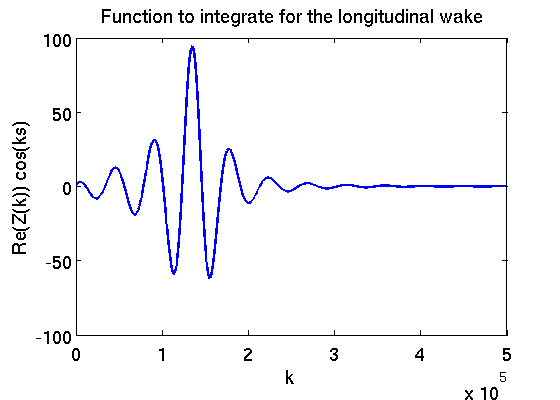
\includegraphics[width=0.45\textwidth]{wakeComp/lo_Integration.png}
%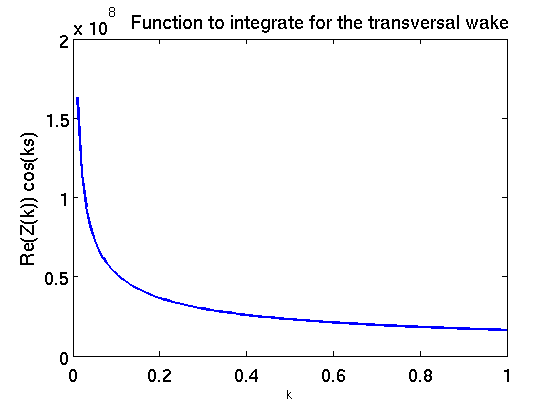
\includegraphics[width=0.45\textwidth]{wakeComp/tr_Integration.png}
%\caption{Parameters of the numerical integration scheme: $N$ and $\Delta k$. \textsc{Left:} longitudinal and \textsc{Right:} transversal wake. \label{fig:lo_calc} }
%\end{center}
%\end{figure}

%As shown in equation~\eqref{eq:Calc_Wl} and~\eqref{eq:Calc_Wt} we need to integrate a function to calculate one sampling point of the wakefunction. For the numerical integration equation~\eqref{eq:Calc_Wl} can be written as a sum from $0$ to $N-1$ since $\infty$ can not be covered numerically, and a discrete $\Delta k$ instead of a infinitesimal $dk$:
%\begin{equation}\label{eq:Num_Calc_Wl}
%W_{L}(s)=10^{-12} \dfrac{2c}{\pi}Re\left(\sum_{i=0}^{N-1} Re(Z_{L}(i \Delta k))\cos (i\Delta ks)dk\right)
%\end{equation}
%with $Re(Z_{L})$ either $Z_{Ldc}$ or $Z_{Lac}$.
%The same holds for equation~\eqref{eq:Calc_Wt} which is then written as
%\begin{equation}\label{eq:Num_Calc_Wt}
%W_{T}(s)=10^{-12} \dfrac{2c}{\pi}Re\left(\sum_{i=0}^{N-1} Re(\frac{c}{k} Z_{L}(i \Delta k))\cos (i\Delta ks)dk\right).
%\end{equation}
%To have reliable results out of equation~\eqref{eq:Num_Calc_Wl} and~\eqref{eq:Num_Calc_Wt} $N$ the number of sampling points must be big enough and $\Delta k$ the mesh size small enough.
%Figure~\eqref{fig:lo_calc} trites to give an intuition how $N$ and $\Delta k$ should be chosen. In the figure the parameters are shwn for a round, copper beam pipe with radius $5$\,mm. In figure~\eqref{fig:lo_calc}  $Re(Z_{Ldc}(k))\cos (ks)$ with $s$=120 $\mu$m is plotted with respect to k. This equation is integrated in equation~\eqref{eq:Num_Calc_Wl} to get the longitudinal wakefield. There it is obvious that k must be at least in the order of $10^5$. In figure~\eqref{fig:tr_calc} $Re(\frac{c}{k}Z_{Lac}(k))\cos (ks)$ with $s$=120 $\mu$m is plotted with respect to k. This equation is integrated according to equation~\eqref{eq:Num_Calc_Wt} to get the transversal wakefield. Figure shows a singularity at k=0. To integrate such functions a small $\Delta k$ (fine mesh) is needed. 

To calculate the integrals in (\ref{eq:Calc_Wl}) and (\ref{eq:Calc_Wt}) numerically the Simpson integration schema with equidistant mesh spacings is applied. This leads to an integration with small $\Delta k$ with a big $N$ which is computational not optimal with respect to efficiency. Since we calculate the wakefield usually just once in the initialization phase the overall performance will not be affected from this.

\section{Wakefield Command} 
\label{sec:wakefieldcmd}
\textbf{NOTE: Currently when using wakefields the domain can only be parallelized in $z$-direction! Please adapt the parallelization in the FieldSolver accordingly}
\begin{verbatim}
Fs1:FIELDSOLVER, FSTYPE = FFT, 
       MX = 32, MY = 32, MT = 32,
        PARFFTX = false, PARFFTY = false, PARFFTT = true,
        BCFFTX = open, BCFFTY = open, BCFFTT = open,
        BBOXINCR = 0, GREENSF = INTEGRATED;
\end{verbatim}

\begin{table}[ht] \tiny
  \begin{center}
    \begin{tabular}{|l|p{0.6\textwidth}|l|}
      \hline
      Command &Purpose \\
      \hline
      \tabline{WAKE}{Specify a wakefield}{wakefield}
      \tabline{TYPE}{Specify the wake function [1D-CSR, LONG-SHORT-RANGE, TRANSV-SHORT-RANGE, LONG-TRANSV-SHORT-RANGE]}{WTYPE}
      \tabline{NBIN}{Number of bins used in the calculation of the line density}{NBIN}
      \tabline{CONST\_LENGTH}{TRUE if the length of the bunch is considered to be constant}{CONSTLEN}
      \tabline{CONDUCT}{Conductivity [AC, DC]}{CONDUCT}
      \tabline{Z0}{Impedance of the beam pipe in [$\Omega$]}{Z}
      \tabline{FORM}{The form of the beam pipe [ROUND]}{FROM}
      \tabline{RADIUS}{The radius of the beam pipe in [m]}{RADIUS}
      \tabline{SIGMA}{Material constant dependent on the beam pipe material in [$\Omega^{-1} m$]} {SIGMA}
      \tabline{TAU}{Material constant dependent on the beam pipe material in [$s$]}{TAU}
      \tabline{FNAME}{Specify a file that provides a wakefunction}{WFNAME}
      \hline
    \end{tabular}
    \caption{Wakefield command summary}
    \label{tab:wakefieldcmd}
  \end{center}
\end{table}

\section{Define the Wakefield to be used}
\label{sec:wakefield}
\index{WAKE}
The WAKE statement defines data for a wakefunction on an element.

\section{Define the wakefield type}
\label{sec:WTYPE}
\index{WTYPE}
Used to specify the wakefunction

\section{Define the number of bins}
\label{sec:NBIN}
\index{NBIN}
The number of bins used in the calculation of the line density.

\section{Define the bunch length to be constant}
\label{sec:CONSTLEN}
\index{CONST_LENGTH}
With the \texttt{CONST\_LENGTH} flag the bunch length can be set to be constant.

\section{Define the conductivity}
\label{sec:CONDUCT}
\index{CONDUCTIVITY}
The conductivity of the bunch which can be set to either AC or DC.

\section{Define the impedance}
\label{sec:Z}
\index{Z0}
The impedance $Z_0$ of the beam pipe in [$\Omega$].

\section{Define the form of the beam pipe}
\label{sec:FROM}
\index{FROM}
The form of the beam pipe can be set to ROUND.

\section{Define the radius of the beam pipe}
\label{sec:RADIUS}
\index{RADIUS}
The radius of the beam pipe in [m].

\section{Define the $\sigma$ of the beam pipe}
\label{sec:SIGMA}
\index{SIGMA}
The $\sigma$ of the beam pipe (material constant), see (\ref{eq:dc_cond}).

\section{Define the relaxation time ($\tau$) of the beam pipe}
\label{sec:TAU}
\index{TAU}
The $\tau$ defines the relaxation time and is needed to calculate the impedance of the beam pipe (see \ref{eq:dc_cond}).

\section{Import a wakefield form a file}
\label{sec:WFNAME}
\index{FNAME}

Since we only need values of the wakefunction at several discreet points to calculate the force on the particle it is also possible to specify these in a file.To get required datapoints of the wakefield not provide in the file we linearly interpolate the available function values. The files are specified in the SDDS\footnote{\url{http://www.aps.anl.gov/Accelerator_Systems_Division/Operations_Analysis/manuals/GettingStartedWithSDDS/HTML/GettingStartedWithSDDS.html}} (Self Describing Data Sets).

Whenever a file is specified \opal will use the wakefield found in the file and ignore all other commands related to round beam pipes.
